\section*{Problema 5}

\textbf{
    El tiempo de ejecucion de algoritmo A es $\mathcal{N}$(2, 1) y de algoritmo B es $\mathcal{N}$(4, 2). Si los tiempos son independientes entre sí, calcula la probabilidad que en una corrida B es más rapido que A.
}

La probabilidad que el algoritmo B obtenga un tiempo menor que A es definida como $P(B<A)$. Sea C el conjunto de valores que toma la variable aleatoria X tal que:

\begin{equation*}
    C=\{x\in X : \mathcal{N}(x,4,2)<\mathcal{N}(x,2,1)\}
\end{equation*}

Encontrando el conjunto de C, se tiene lo siguiente:

\begin{align}
    \frac{1}{\sigma_1 \sqrt{2\pi}} exp\left(-\frac{(x-\mu_1)^2}{2\sigma_1^2}\right) & = \frac{1}{\sigma_2 \sqrt{2\pi}} exp\left(-\frac{(x-\mu_2)^2}{2\sigma_2^2}\right)                               \nonumber                     \\
    -ln\left(\sigma_1 \sqrt{2\pi}\right) -\frac{(x-\mu_1)^2}{2\sigma_1^2}           & = -ln\left(\sigma_2 \sqrt{2\pi}\right) -\frac{(x-\mu_2)^2}{2\sigma_2^2}                                         \nonumber                     \\
    \frac{(x-\mu_2)^2}{2\sigma_2^2} -\frac{(x-\mu_1)^2}{2\sigma_1^2}                & =ln\left(\sigma_1 \sqrt{2\pi}\right) - ln\left(\sigma_2 \sqrt{2\pi}\right)                                      \nonumber                     \\
    \sigma_1^2(x-\mu_2)^2 -\sigma_2^2(x-\mu_1)^2                                    & = 2 \sigma_1^2 \sigma_2^2 ln\left(\frac{\sigma_1}{\sigma_2}\right)                                              \nonumber                     \\
    (\sigma_1^2-\sigma_2^2) x^2 + 2(\mu_1\sigma_2^2-\mu_2\sigma_1^2) x              & + \sigma_1^2 \mu_2^2 - \sigma_2^2 \mu_1^2 - 2 \sigma_1^2 \sigma_2^2 ln\left(\frac{\sigma_1}{\sigma_2}\right) =0 \label{eq:quatratic_problem5}
\end{align}

donde la ecuación \ref{eq:quatratic_problem5} es una ecuación cuadratica. Tomando en cuenta los parametros $\mu_1=2$, $\sigma_1 = 1$, $\mu_2= 4$ y $\sigma_2=2$, las soluciones son $x=\{-3.063706,3.063706\}$. Como las distribuciones representan tiempos, entonces las solución negativa será despreciada. Por lo que la el conjunto C puede ser escrito como:

\begin{equation*}
    C=\{x\in X : 0<x<3.063706\}
\end{equation*}

Entonces

\begin{align}
    P(B<A) & = P(0<x<3.063706)                                        \\
    P(B<A) & = P(x<3.063706) - P(x<0) \label{eq:probability_problem5}
\end{align}

La probabilidad señalada en la ecuación \ref{eq:probability_problem5} es la señalada en la figura \ref{fig:probability_problem5}.

\begin{figure}[H]
    \centering
    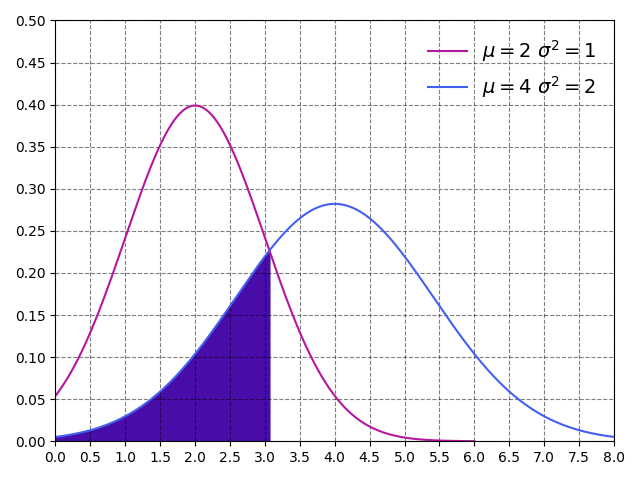
\includegraphics[width=10cm]{Graphics/problem5.png}
    \caption{Área a integrar en la ecuación \ref{eq:quatratic_problem5}.}
    \label{fig:probability_problem5}
\end{figure}

Por lo tanto

\begin{align*}
    P(B<A) & = P(x<3.063706) - P(x<0) \\
           & = 0.3198396 - 0.02275013 \\
    P(B<A) & = 0.2970894
\end{align*}